\section{The Expectation-Maximization (EM) algorithm}

\begin{frame} 
\mode<presentation>{
    \begin{center} \huge
        \secname
    \end{center}
    }    
    \begin{itemize}
       \item \textbf{What}: iterative learning method that alternates between two-steps\\ (E and M-step)\\
       \item \textbf{Goal}: approximate maximization of the likelihood function
    \end{itemize}
	
\end{frame}

\begin{frame}{\secname}
    \begin{itemize}
		\item We've seen EM in clustering, Self-Organizing Maps and density estimation.
	   \item Latent variable models: an abstraction of Gaussian Mixture Models
    \end{itemize}
\end{frame}

\subsection{Example scenario}

\begin{frame}{\subsecname}

\svspace{-5mm}

\question{What is the distribution of shoe sizes in Berlin?}

\svspace{-5mm}

\begin{center}
\slidesonly{
	\includegraphics<1>[width=0.45\textwidth]{img/latentexample_nofit}
	}
	\includegraphics<2>[width=0.45\textwidth]{img/latentexample}
	\includegraphics<3->[width=0.45\textwidth]{img/latentexamplekde}
\end{center}

\svspace{-3mm}

\pause 

We recognize two sub-groups in the data. There are \emph{hidden causes} in the observations. We need a better fit that:

\pause

\begin{enumerate}
\item increases the resolution of our parametric density estimation (we want to continue using Gaussians),
\item estimates densities around each \underline{unknown} group
\end{enumerate}

\end{frame}

\subsection{Latent variable models}

\begin{frame}{Latent variable models}

\begin{center}
	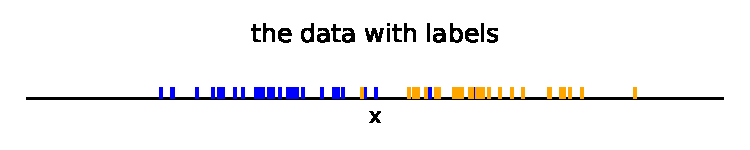
\includegraphics[width=0.8\textwidth]{img/latentexample_nofit_labels}
	\notesonly{\captionof{figure}{The labeling of points according to the group which we do not have.}}
\end{center}

We don't have any labels for the data and no access to the hidden causes. However, we can model these causes using latent variables.

\end{frame}

\begin{frame}{Assignment variables as latent variables}

A simple way to understand what latent variables represent is to view them as assignment variables to components that we need to estimate.

Example:\\

\begin{itemize} 
\item assignment variables: $\vec{m}^{(\alpha)} =  \big( m_1^{(\alpha)}, \dots, m_M^{(\alpha)} \big)^\top \in \left\{ 0, 1 \right\}^M$ \\
		\begin{align}
		m_q^{(\alpha)} &= 
		\begin{cases}
		1, & \text{if component } q \text{ has generated point}~\alpha\\
		0, & \text{otherwise}
		\end{cases}
		%\hspace{0.5cm}
		\;\text{with} \;
		 \sum_{q=1}^{M} m_q^{(\alpha)} = 1 
		\end{align}
\end{itemize}

\svspace{-7mm}

\notesonly{We have also seen how Gaussian Mixture Models can model assignment variables using mixture components.}

\begin{center}
	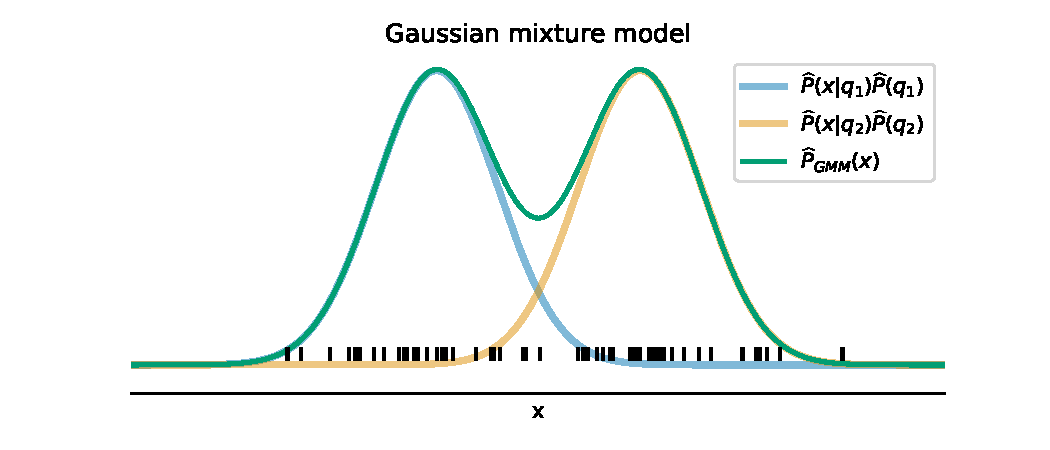
\includegraphics[width=0.7\textwidth]{img/latentexample_gmm}
	\notesonly{\captionof{figure}{A Gaussian Mixture Model as a latent variable model}}
\end{center}


\end{frame}

%\subsection{Approximating MLE using EM}

\begin{frame}{Maximum Likelihood Estimation (MLE)}

Let $\{ \vec x^{(\alpha)}\}$ denote the entire dataset with $p$ observations.

    \begin{equation}
		\widehat P(\{ \vec x^{(\alpha)} \} | \vec w) \;\; \stackrel{\text{iid}}{=} \;\; \prod_{\alpha=1}^p \widehat P(\vec x^{(\alpha)} | \vec w) \; \eqexcl \; \max_{\vec w}
    \end{equation}
    
Equivalent to minimizing the negative log likelihood:

    \begin{equation}
    - \ln \widehat P(\{ \vec x^{(\alpha)} \} | \vec w) \;\; \stackrel{\text{iid}}{=} \;\; 
		- \sum_{\alpha=1}^p \ln \widehat P(\vec x^{(\alpha)} | \vec w) \; \eqexcl \; \min_{\vec w}
    \end{equation}

	
\end{frame}

\begin{frame}{Latent variable models}

\notesonly{Latent variable models}\slidesonly{We} view the data likelihood as a \textcolor{blue}{marginalization} of the latent variables:

\svspace{-1mm}

\begin{equation}
P \left( \left\{ \vec{x}^{(\alpha)} \right\} | \vec{w} \right) \stackrel{\text{iid}}{=} \prod_{\alpha=1}^{p} P \left( \vec{x}^{(\alpha)} | \vec{w} \right) = \prod_{\alpha=1}^{p}  
\kern-4ex
\underbrace{{\color{blue}\sum_{\vec{m}}}}_{
\substack{\text{all possible}\\\text{valid assignments}\\{\text{for point }\alpha}}
} 
\kern-4ex
P \left( \vec{x}^{(\alpha)}, \vec{m} | \vec{w} \right)
\end{equation}

\svspace{-5mm}

The corresponding log-likelihood:

\begin{equation}
\ln P \left( \left\{ \vec{x}^{(\alpha)} \right\} | \vec{w} \right) = \sum_{\alpha=1}^{p}  \ln \left( {\color{blue}\sum_{\vec{m}}} P \left( \vec{x}^{(\alpha)}, \vec{m} | \vec{w} \right) \right)
\end{equation}

The sum in the logarithm prevents us from finding a closed-form solution.

\pause

\slidesonly{
\svspace{-1mm}

\begin{center}
	
\includegraphics[width=0.3\textwidth]{img/meme_emrescue}
\end{center}
}

\end{frame}

\subsection{The EM algorithm}

\begin{frame}{\subsecname}


The objective is to maximize the likelihood of the data.\\

The EM algorithm is an iterative approximate solution to maximizing the likelihood for a problem that requires \emph{alternation}.

\end{frame}

\begin{frame}{\subsecname}

\begin{block}{The need to alternate}

We need to know who is assigned to which group in order to estimate the density of that group (i.e. identify which data influences a component $q$)\\
\textbf{But} we don't know the assignments.\\
To get the assignments we need the density of that group\ldots\\

Modifying one will lead to a modification of the other.

\end{block}

\pause

\begin{center}
\begin{minipage}{0.1\textwidth}
\begin{center}
	
\includegraphics[width=0.9\textwidth]{img/fried-chicken}
\end{center}
\end{minipage}
\begin{minipage}{0.1\textwidth}
\begin{center}
	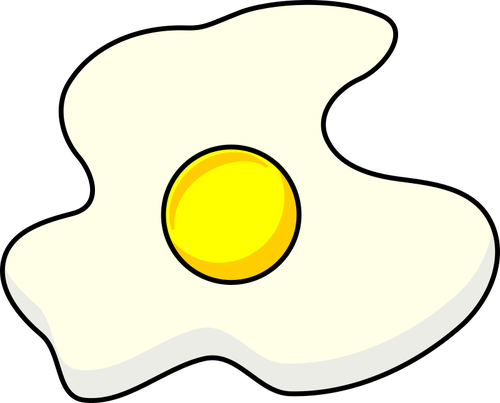
\includegraphics[width=0.9\textwidth]{img/fried-egg}
\end{center}
\end{minipage}
\end{center}

\pause

\question{Where have we encountered this alternating behavior before?}

- K-means. But there we didn't dwell too much about any chicken-and-egg problem. Basing everything on Euclidean distance took care of this.


\end{frame}

\begin{frame}

\slidesonly{
\begin{center}
	
\includegraphics[width=0.5\textwidth]{img/meme_cycle}
\end{center}
}

\end{frame}


%%%%%%%%%%%%%%%%%%%%%%%%%%%%%%%%%%%%%%%%%%%%%%%%%%%%%%
\begin{frame}{\subsecname: Outline}

\begin{figure}[!th]
\footnotesize
\removelatexerror
\small
\scalebox{.9}{   
	\begin{algorithm}[H]
		\DontPrintSemicolon
		initialization:\\
		Decide on the number of groups.
		Random initial densities (i.e. random initialization of density parameters)\\
		\vspace{1mm}
		\Repeat{change below tolerance}{
			\vspace{3mm}
			1. \textbf{E-step}: Use the densities to assign points to groups\\
			
			\vspace{3mm}
			2. \textbf{M-step}: Use the current assignments to update the densities\\
			\vspace{3mm}
		}
		\caption{Outline of the EM algorithm}
	\end{algorithm}
}
\end{figure}

\pause

\slidesonly{
\begin{center}
	
\includegraphics[width=0.3\textwidth]{img/meme_kmeans}
\end{center}
}

\notesonly{
If you find that the outline of the EM algorithm looks a lot like K-means, it's because K-means is a special case of EM.
}


\end{frame}

\subsection{Does EM work?}

\begin{frame}{\subsecname}

We now need reassurance that alternating between the steps improves both
\begin{itemize}
\item[A] our assignments\\
AND\\
\item[B] our densities
\end{itemize}

\end{frame}

\begin{frame}{\subsecname}

\begin{itemize}
\item observed variables $\vec x \in \R^N$
\item latent (hidden) variables $\vec m \in \R^M$
\item Parameters of the densities we want to estimate: $\vec w$ (e.g. $\vec \mu$, $\sigma^2$ for every Gaussian component $q$)
\end{itemize}

\textbf{Objetive}: Maximize the joint distribution of observed and latent variables with $p$ samples:
\begin{align}
	\widehat{P} \left( \vec x^{(1)}, \vec x^{(2)},\ldots, \vec x^{(p)}, \vec m^{(1)}, \vec m^{(2)},\ldots, \vec m^{(p)}~|~\vec w \right) \eqexcl \max_{\vec w}\\
	\widehat{P} \left( \{\vec x^{(\alpha)}\}, \{\vec m^{(\alpha)}\}~|~\vec w \right) \eqexcl \max_{\vec w}~, \;\; \alpha=1,\ldots,p
\end{align}

$\vec w$ depend on the assignments $\vec m$ but these are unknown.

\pause

\question{How do $\vec x$, $\vec m$ and $\vec w$ interact with one another?}

\end{frame}

\begin{frame}{How do $\vec x$, $\vec m$ and $\vec w$ interact with one another?}

\svspace{-2mm}

We start with the likelihood function:

\svspace{-5mm}

\begin{align}
	\widehat{P} \left( \{\vec x^{(\alpha)}\}~|~\vec w \right)
	&\stackrel{\text{iid}}{=}
	\prod_{\alpha=1}^{p}  \widehat{P} \left( \vec x^{(\alpha)}~|~\vec w \right)
	\intertext{``\textcolor{blue}{sum out}'' the latent variables to recover the likelihood}
	&= \prod_{\alpha=1}^{p} {\color{blue}\sum_{\vec m}} \widehat{P} \left( \vec x^{(\alpha)}, \vec m~|~\vec w \right)
\end{align}

\pause

\begin{equation}
P(a,b) = P(a|b)~P(b) \qquad \text{(product rule)}
\end{equation}

From this follows {\footnotesize(omitting indices for readability)}:

\svspace{-5mm}

\begin{align}
P(~\vec x,\vec m ~|~ \vec w) &= P(~\vec x~|~\vec m;\vec w)~P(\vec m~|~ \vec w)\\
P(~\vec m, \vec x ~|~ \vec w) &= P(~\vec m~|~\vec x;\vec w)~P(\vec x~|~ \vec w)
\end{align}

It does not matter how we order the arguments of a joint distributions:

\svspace{-3mm}

\begin{equation}
P(~\vec x,\vec m ~|~ \vec w) = P(~\vec m, \vec x ~|~ \vec w)
\end{equation}

\end{frame}

\begin{frame}{How do $\vec x$, $\vec m$ and $\vec w$ interact with one another?}

\svspace{-3mm}

\slidesonly{
\begin{flushright}
{\footnotesize (omitting indices for readability)}\\
\end{flushright}
}

\svspace{-7mm}

\slidesonly{
\begin{align}
P(~\vec m, \vec x ~|~ \vec w) &= P(~\vec m~|~\vec x;\vec w)~P(\vec x~|~ \vec w)
\end{align}
}

%\begin{align}
%\widehat{P}(~\vec x,\vec m ~|~ \vec w) &= \widehat{P}(~\vec m, \vec x ~|~ \vec w)\\
%\widehat{P}(~\vec x~|~\vec m;\vec w)~\widehat{P}(~\vec m ~|~ \vec w) &=
%\widehat{P}(~\vec m~|~\vec x;\vec w)~\widehat{P}(~\vec x ~|~ \vec w)\\
%\end{align}

%\svspace{-5mm}

\pause

%\svspace{-5mm}

%Plugging $\widehat{P}(~\vec m, \vec x ~|~ \vec w) = \overbrace{\widehat{P}(~\vec m~|~\vec x;\vec w)}^{\text{posterior}}~\widehat{P}(~\vec x ~|~ \vec w)$ into the likelihood.

%\pause

%We've stablished that the likelihood is recovered by marginalizing over the latent variables.

%\svspace{-3mm}

%\begin{align}
	%\widehat{P} \left(~\vec x~|~\vec w \right)
	%&= \sum_{\vec m} \widehat{P} \left(~\vec x, \vec m~|~\vec w \right)\\
	%&= \sum_{\vec m} \widehat{P}(~\vec x~|~\vec m;\vec w)~\widehat{P}(~\vec m ~|~ \vec w)\\
	%\text{equivalently}
	%&= \sum_{\vec m} \widehat{P}(~\vec m~|~\vec x;\vec w)~\widehat{P}(~\vec x ~|~ \vec w)\\
%\end{align}

%Posterior distribution of latent variables $\vec m$ given observations $\vec x$:

%\begin{align}
%\widehat{P}(~\vec m~|~\vec x;\vec w) &= \frac{\widehat{P}(~\vec m, \vec x ~|~ \vec w)}{\widehat{P}(~\vec x ~|~ \vec w)}\\
%\widehat{P}(~\vec x ~|~ \vec w) &= \frac{\widehat{P}(~\vec m, \vec x ~|~ \vec w)}{\widehat{P}(~\vec m~|~\vec x;\vec w)}
%\end{align}

This gives us an alternative expression for the likelihood function:

\begin{equation}
\widehat{P}(~\vec x ~|~ \vec w) = \frac{\widehat{P}(~\vec m, \vec x ~|~ \vec w)}{\widehat{P}(~\vec m~|~\vec x;\vec w)}
\end{equation}

We introduce $P(\vec m)$ as the prior distribution of latent variables $\vec m$. No need to define it just yet:

\svspace{-7mm}

\slidesonly{
\begin{align}
\widehat{P}(~\vec x ~|~ \vec w) &= \frac{\widehat{P}(~\vec m, \vec x ~|~ \vec w)}{\widehat{P}(~\vec m~|~\vec x;\vec w)}
~\cdot~
\frac{P(\vec m)}{P(\vec m)}
\end{align}
}

\end{frame}

\begin{frame}{How do $\vec x$, $\vec m$ and $\vec w$ interact with one another?}

\only<1,2>{
\begin{align}
\widehat{P}(~\vec x ~|~ \vec w) &= \frac{\widehat{P}(~\vec m, \vec x ~|~ \vec w)}{\widehat{P}(~\vec m~|~\vec x;\vec w)}
~\cdot~
\frac{P(\vec m)}{P(\vec m)}\\
&= \frac{{\widehat{P}(~\vec m, \vec x ~|~ \vec w)} \cdot P(\vec m)}{P(\vec m) \cdot \widehat{P}(~\vec m~|~\vec x;\vec w)}\\
%&= \frac{{\color{blue}\widehat{P}(~\vec x~|~\vec m;\vec w)~\widehat{P}(~\vec m ~|~ \vec w)} \cdot P(\vec m)}{\cdot P(\vec m) \widehat{P}(~\vec m~|~\vec x;\vec w)}\\
%&= \frac{{\color{blue}\widehat{P}(~\vec x~|~\vec m;\vec w)~\widehat{P}(~\vec m ~|~ \vec w)} \cdot P(\vec m)}{\cdot P(\vec m) \widehat{P}(~\vec m~|~\vec x;\vec w)}\\
&= \frac{\widehat{P}(~\vec m, \vec x ~|~ \vec w)}{P(\vec m)} \cdot \frac{P(\vec m)}{\widehat{P}(~\vec m~|~\vec x;\vec w)}
\end{align}

We take the logarithm on both sides
}

\only<2-3>{
\begin{equation}
\ln \widehat{P}(~\vec x ~|~ \vec w)
= \ln \frac{\widehat{P}(~\vec m, \vec x ~|~ \vec w)}{P(\vec m)} + \ln \frac{P(\vec m)}{\widehat{P}(~\vec m~|~\vec x;\vec w)}
\end{equation}
}

\only<3->{
Compute the expectation w.r.t. $P(\vec m)$:

\only<4->{
\slidesonly{
\begingroup
\small
}
}
\begin{align}
\E
\big\lbrack
\ln \widehat{P}(~\vec x ~|~ \vec w)
\big\rbrack
&= \int P(\vec m) \ln  \frac{\widehat{P}(~\vec m, \vec x ~|~ \vec w)}{P(\vec m)} d\vec m \\
&\;\;+ \int P(\vec m) \ln \frac{P(\vec m)}{\widehat{P}(~\vec m~|~\vec x;\vec w)} d\vec m
\end{align}
\only<4->{
\slidesonly{
\endgroup
}
}

}

\only<4>{
\question{How did we get here?}

- likelihood $\rightarrow$ product rule $\rightarrow$ $P(\vec m)$ $\rightarrow$ log $\rightarrow$ $\E\lbrack \cdot \rbrack$

}

\only<5->{

\question{What is all this for?}

\begin{itemize}
\item[-] We want to see if EM can actually maximize the likelihood
\item[-] To do so, we need to see how the different variables interact
\item[-] This lets us formulate the terms that EM uses during the optimization
\item[-] Bonus: We find a hint to what \emph{Expectation} is actually \emph{maximized}
\end{itemize}
}

\end{frame}

\begin{frame}{\subsecname}

\svspace{-5mm}

\question{What do the terms in the expectation represent?}

\svspace{-5mm}

\begingroup
\small
\begin{align}
\E
\big\lbrack
\ln \widehat{P}(~\vec x ~|~ \vec w)
\big\rbrack
&= \int P(\vec m) \ln \frac{\widehat{P}(~\vec m, \vec x ~|~ \vec w)}{P(\vec m)} d\vec m 
\;+ \int P(\vec m) \ln \frac{P(\vec m)}{\widehat{P}(~\vec m~|~\vec x;\vec w)} d\vec m\slidesonly{\\[-7mm]}
\intertext{\footnotesize switching numerator and denominator in second integral adds a minus sign in front of the integral}
&= \int P(\vec m) \ln  \frac{\widehat{P}(~\vec m, \vec x ~|~ \vec w)}{P(\vec m)} d\vec m
~
{\color{red}-} \int P(\vec m) \ln \frac{\color{red}\widehat{P}(~\vec m~|~\vec x;\vec w)}{\color{red}P(\vec m)} d\vec m \\ 
&= 
\underbrace{\int P(\vec m) \ln \frac{\widehat{P}(~\vec m, \vec x ~|~ \vec w)}{P(\vec m)} d\vec m
}_{\substack{=:~\mathscr{L}(P(\vec m), \vec w)\\\text{the expected complete}\\\text{data log-likelihood}}}
\,
\underbrace{-\int P(\vec m) \ln \frac{\widehat{P}(~\vec m~|~\vec x;\vec w)}{P(\vec m)} d\vec m
}_{+\dkl \left\lbrack P(\vec m) ~||~ P(~\vec m~|~ \vec x; \vec w) \right\rbrack}
\end{align}
\endgroup

\end{frame}

\begin{frame}{Verifying the decomposition}

\notesonly{Before we continue let's verify the decomposition from before:}

\begingroup
\small
\begin{align}
\E
\big\lbrack
\ln \widehat{P}(~\vec x ~|~ \vec w)
\big\rbrack
&= 
\mathscr{L}(P(\vec m), \vec w) + {\color{red}\dkl \left\lbrack P(\vec m) ~||~ P(~\vec m~|~ \vec x; \vec w) \right\rbrack}\\
&= 
\int P(\vec m) \ln \frac{\widehat{P}(~\vec m, \vec x ~|~ \vec w)}{P(\vec m)} d\vec m
+ 
{\color{red}\dkl}\\
&= 
\int P(\vec m) \ln \frac{\widehat{P}(~\vec m ~|~ \vec x ; \vec w) \widehat{P}(~\vec x ~|~ \vec w)}{P(\vec m)} d\vec m
+ 
{\color{red}\dkl}\\
&= 
\int P(\vec m) \ln \frac{{\color{blue}\widehat{P}(~\vec m ~|~ \vec x ; \vec w)} \widehat{P}(~\vec x ~|~ \vec w)}{{\color{blue}P(\vec m)}} d\vec m
+
{\color{red}\dkl}\\
&= 
\int P(\vec m) \ln \widehat{P}(~\vec x ~|~ \vec w) d\vec m
+\kern-0.7ex
\int \kern-0.5ex P(\vec m) \ln \frac{{\color{blue}\widehat{P}(~\vec m ~|~ \vec x ; \vec w)}}{{\color{blue}P(\vec m)}} d\vec m
+
{\color{red}\dkl}\\
&= 
\int P(\vec m) \ln \widehat{P}(~\vec x ~|~ \vec w) d\vec m
~{\color{red} - \dkl}
+
{\color{red}\dkl}\\
&= \E
\big\lbrack
\ln \widehat{P}(~\vec x ~|~ \vec w)
\big\rbrack
\end{align}
\endgroup

\end{frame}

\begin{frame}{\subsecname}

\question{What do we gain from this decomposition?}

\slidesonly{
\begingroup
\footnotesize
\begin{align}
\E
\big\lbrack
\ln \widehat{P}(~\vec x ~|~ \vec w)
\big\rbrack
&= 
\mathscr{L}(P(\vec m), \vec w) + {\dkl \left\lbrack P(\vec m) ~||~ P(~\vec m~|~ \vec x; \vec w) \right\rbrack}
\end{align}
\endgroup
}

\pause

- We use the decomposition to show how EM optimizes the log likelihood at every iteration.

\end{frame}

\begin{frame}{\subsecname}

\svspace{-5mm}

\slidesonly{
\begingroup
\footnotesize
\begin{align}
\E
\big\lbrack
\ln \widehat{P}(~\vec x ~|~ \vec w)
\big\rbrack
&= 
\mathscr{L}(P(\vec m), \vec w) + {\dkl \left\lbrack P(\vec m) ~||~ P(~\vec m~|~ \vec x; \vec w) \right\rbrack}
\end{align}
\endgroup
}


\begin{block}{Jensen's inequality}

Given a random variable $Z$, Jensen's inequality tells us that for any convex function $f$:

\slidesonly{
\placeimage{12.5}{4}{img/convex}{width=2cm}
}

\svspace{-5mm}

\begin{equation}
f(\E[Z]) \leq \E[f(Z)]    
\end{equation}
  
\pause

The reverse is true for a concave function $g$:
  
\begin{equation}
g(\E[Z]) \geq \E[g(Z)]    
\end{equation}

\end{block}

\notesonly{
\begin{center}
\begin{minipage}{0.2\textwidth}
\begin{center}
	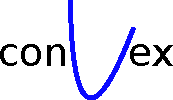
\includegraphics[width=0.9\textwidth]{img/convex}
\end{center}
\end{minipage}
\begin{minipage}{0.2\textwidth}
\begin{center}
	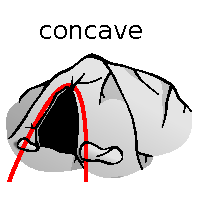
\includegraphics[width=0.9\textwidth]{img/concave}
\end{center}
\end{minipage}
\end{center}
}

\slidesonly{
\placeimage{12}{7}{img/concave}{width=2cm}
}

\pause

\svspace{5mm}

The logarithm $\ln(z)$ is concave in the interval $0 < z < \infty$.
The derivative $\frac{d \ln(z)}{dz} = \frac{1}{z}$ strictly decreases when its argument increases.

\pause

\question{What does this have to do with anything?}

\notesonly{
- It tells us that $\E \big\lbrack \ln \widehat{P}(~\vec x ~|~ \vec w) \big\rbrack$ has a lower bound.
}


\end{frame}

\begin{frame}{The lower bound}

\slidesonly{
\begingroup
\footnotesize
\begin{align}
\E
\big\lbrack
\ln \widehat{P}(~\vec x ~|~ \vec w)
\big\rbrack
&= 
\mathscr{L}(P(\vec m), \vec w) + {\dkl \left\lbrack P(\vec m) ~||~ P(~\vec m~|~ \vec x; \vec w) \right\rbrack}
\end{align}
\endgroup
}

Since $\dkl \ge 0$ and $\dkl = 0$ iff. $P(\vec m) = P(~\vec m~|~ \vec x; \vec w)$, the expected complete data log-likelihood $\mathscr{L}(P(\vec m), \vec w)$ is a lower bound on $\E
\big\lbrack
\ln \widehat{P}(~\vec x ~|~ \vec w)
\big\rbrack$.

\pause

\begin{enumerate}[a]
\item The EM algorithm maximizes the log-likelihood by maximizing the lower bound $\mathscr{L}(P(\vec m), \vec w)$ at every iteration $t$ w.r.t. $P(\vec m)$.
\item With every increase the $\dkl$ term becomes smaller and \underline{may} eventually vanish.
\item In the case of the $\dkl$ term vanishing, $\mathscr{L}(P(\vec m), \vec w) = \E
\big\lbrack
\ln \widehat{P}(~\vec x ~|~ \vec w)
\big\rbrack$
\item The likelihood under EM is strictly monotonically increasing. \notesonly{During intermediate optimization steps in EM lead to the likelihood increasing or remaining unchanged.}
\item A decrease is indicative of a mistake in the implementation.
\end{enumerate}

\end{frame}

%\begin{frame}{\subsecname}

%\slidesonly{
%\begingroup
%\scriptsize
%\begin{align}
%\E
%\big\lbrack
%\ln \widehat{P}(~\vec x ~|~ \vec w)
%\big\rbrack
%&= 
%\mathscr{L}(P(\vec m), \vec w) + {\dkl \left(~P(\vec m) ~||~ P(~\vec m~|~ \vec x; \vec w) ~\right)}
%\end{align}
%\endgroup
%}

%\end{frame}

\subsection{How does EM work?}

\subsubsection{The E-step}

\begin{frame}{\subsubsecname}

\svspace{-3mm}

\begin{center}
	\includegraphics[width=0.6\textwidth]{img/emconverge}
	\notesonly{
	\captionof{figure}{Illustration of the convergence of EM to a local maximum}
	}
\end{center}

\svspace{-5mm}

\slidesonly{
\begingroup
\scriptsize
\begin{align}
\E
\big\lbrack
\ln \widehat{P}(~\vec x ~|~ \vec w)
\big\rbrack
&= 
\mathscr{L}(P(\vec m), \vec w) + {\dkl \left\lbrack P(\vec m) ~||~ P(~\vec m~|~ \vec x; \vec w) \right\rbrack}
\end{align}
\endgroup
}

\svspace{-5mm}

\begin{enumerate}
\item Maximize $\mathscr{L}(P(\vec m), \vec w)$ w.r.t. $P(\vec m)$ keeping the parameters fixed (i.e. use $\vec w_{\text{old}}$)
\item At the solution the $\dkl$ decreases (ultimately, $\dkl \rightarrow$ 0)
\end{enumerate}

\end{frame}

\subsubsection{The M-step}

\begin{frame}{\subsubsecname}

\svspace{-3mm}
\slidesonly{
\only<1>{
\begin{center}
	\includegraphics[width=0.6\textwidth]{img/emconverge}
\end{center}

\svspace{-5mm}
}

\begingroup
\scriptsize
\begin{align}
\E
\big\lbrack
\ln \widehat{P}(~\vec x ~|~ \vec w)
\big\rbrack
&= 
\mathscr{L}(P(\vec m), \vec w) + {\dkl \left\lbrack P(\vec m) ~||~ P(~\vec m~|~ \vec x; \vec w) \right\rbrack}
\end{align}
\endgroup
}

\svspace{-5mm}

\begin{enumerate}
\item Keep $P(\vec m)$ fixed.
\item Maximize $\mathscr{L}(P(\vec m), \vec w)$ w.r.t. $\vec w \leadsto \vec w_{\text{new}}$

\pause

\item We either manage to increase the lower bound or it remains unchanged
\begin{equation}
\mathscr{L}(P(\vec m), \vec w_{\text{new}}) \ge \mathscr{L}(P(\vec m), \vec w_{\text{old}})
\end{equation}
\item The possible increase in $\mathscr{L}$ leads to an increase in the likelihood but not necessarily by a different amount.\\
The difference in increase is explained by the $\dkl$ term.
\end{enumerate}

\pause

\question{Which of the two will increase more? The likelihood or $\mathscr{L}$?}

\pause

-Since $\dkl \ge 0$, the increase in the likelihood can be larger than that of $\mathscr{L}$.

\end{frame}

\begin{frame}

\question{How should we define $P(\vec m)$?}

- By keeping $P(\vec m)$ fixed during the M-step, we are effectively measuring $P(\vec m)$ as a function of the data \notesonly{and the parameters values of the previous step }$\vec w_{\text{old}}$.

This leads to the following definition

\begin{equation}
P(\vec m) := P(~\vec m ~|~ \vec x ; \vec w_{\text{old}})
\end{equation}

\pause

We revise our definition of the complete data log-likelihood accordingly:

\begingroup
\small
\begin{align}
\mathscr{L}(P(\vec m), \vec w) :=&~\mathscr{L}(P(~\vec m ~|~ \vec x ; \vec w_{\text{old}}), {\color{red}\vec w})\\
=
\int &P(~\vec m ~|~ \vec x ; \vec w_{\text{old}}) \ln \frac{\widehat{P}(~\vec m, \vec x ~|~ {\color{red}\vec w})}{P(~\vec m ~|~ \vec x ; \vec w_{\text{old}})} d\vec m\\
= \kern-0.7ex
\int \kern-0.3ex P(~\vec m ~|~ \vec x ; \vec w_{\text{old}}) \ln &{\widehat{P}(~\vec m, \vec x ~|~ {\color{red}\vec w})}\kern-0.3ex d\vec m
\underbrace{
- \kern-0.7ex \int \kern-0.4ex P(~\vec m ~|~ \vec x ; \vec w_{\text{old}}) \ln {P(~\vec m ~|~ \vec x ; \vec w_{\text{old}})}~d\vec m
}_{
\substack{
\text{entropy of }P(~\vec m ~|~ \vec x ; \vec w_{\text{old}})\\
\text{does not depend on }\vec w ~\Rightarrow ~\text{const.}
}
}
\end{align}
\endgroup

\end{frame}

\begin{frame}

This leaves us with:
\begin{align}
\mathscr{L}(P(~\vec m ~|~ \vec x ; \vec w_{\text{old}}), {\color{red}\vec w})
&=
\int P(~\vec m ~|~ \vec x ; \vec w_{\text{old}}) \ln {\widehat{P}(~\vec m, \vec x ~|~ {\color{red}\vec w})}~d\vec m
\intertext{for a finite dataset with $p$ points and $M$ components (bringing back the indices):}
=
\sum_{\mathscr{M}} 
\sum_{\alpha=1}^p 
 P(~\vec m^{(\alpha)} ~|~ \vec x^{(\alpha)} ; \vec w_{\text{old}}) &\ln {\widehat{P}(~\vec m^{(\alpha)}, \vec x^{(\alpha)} ~|~ {\color{red}\vec w})}~d\vec m
=: \mathcal{Q}(\vec{w}, \vec{w}_{\text{old}})
\end{align}

Here, $\mathscr{M}$ is the set of all possible and valid assignment vectors for all data points.


\end{frame}


%%%%%%%%%%%%%%%%%%%%%%%%%%%%%%%%%%%%%%%%%%%%%%%%%%%%%%
\begin{frame}{The Expectation-Maximization (EM) algorithm}
\begin{figure}[!th]
\footnotesize
\removelatexerror
\small
\scalebox{.9}{   
	\begin{algorithm}[H]
		\DontPrintSemicolon
		Choose initial values for the parameters $\vec{w}_\text{old}$ (e.g., by random)	and tolerance $\theta$\;
		\vspace{1mm}
		\Repeat{$| \vec{w}_\text{old} - \vec{w}_\text{new} | < \theta$}{
			\vspace{3mm}
			1. Compute the posterior distribution: $P \left( \left\{ \vec{m}^{(\alpha)} \right\} \big| \left\{ \vec{x}^{(\alpha)} \right\} , \vec{w}_{\text{old}} \right)$\;
			\vspace{3mm}
			2. E-Step: Compute expectation of complete data log-likelihood \\
						\hspace{1.5cm} w.r.t posterior of $\left\{ \vec{m}^{(\alpha)} \right\}$
			\vspace{-1mm}
			\begin{equation*}
			\mathcal{Q}(\vec{w}, \vec{w}_{\text{old}}) = 
			%\sum_{\left\{ \vec{m}^{(\alpha)} \right\}} 
			\sum_{\mathscr{M}} 
			P \bigg( \big\{ \vec{m}^{(\alpha)} \big\} \big| \big\{ \vec{x}^{(\alpha)} \big\}, \vec{w}_{\text{old}} \bigg) \ln P \bigg( \big\{ \vec{x}^{(\alpha)} \big\}, \big\{ \vec{m}^{(\alpha)} \big\} \big| \vec{w} \bigg)
			\end{equation*}\;
			\vspace{-5mm}
			3. M-Step: Determine new parameters that maximize the expectation
			\vspace{-1mm}
			\begin{align*}
			\vec{w}_{\text{new}} &= \operatorname{arg} \max_{(\vec{w})} \mathcal{Q}(\vec{w}, \vec{w}_{\text{old}}) \\
			\vec{w}_{\text{old}} &\leftarrow \vec{w}_{\text{new}}
			\end{align*}    
		
		}
	\end{algorithm}
	
    \vspace{2mm}
}\\
\slidesonly{
{\footnotesize
$\mathscr{M}$ : Set of all possible and valid assignment vectors for all data points.
}
}
\end{figure}
\end{frame}
